\documentclass[12pt]{article}
%\usepackage[final]{pdfpages}

\usepackage{graphicx}


\usepackage{tikz}
\usetikzlibrary{arrows}

\newcommand{\bbr}{\Bbb{R}}
\newcommand{\zn}{\Bbb{Z}^n}

%\usepackage{epsfig}
%\usepackage{subfigure}
\usepackage{amscd}
\usepackage{amssymb}
\usepackage{amsbsy}
\usepackage{amsthm}
\usepackage{natbib}
\usepackage{amsbsy}
\usepackage{enumerate}
\usepackage{amsmath}
\usepackage{eurosym}
%\usepackage{beamerarticle}
\usepackage{txfonts}
\usepackage{multicol}
\usepackage{fancyvrb}
\usepackage{fancyhdr}
\usepackage{natbib}
\bibliographystyle{chicago}

\usepackage{vmargin}
\usepackage{vmargin}
% left top textwidth textheight headheight
% headsep footheight footskip
\setmargins{2.0cm}{2.5cm}{16 cm}{22cm}{0.5cm}{0cm}{1cm}{1cm}
\renewcommand{\baselinestretch}{1.3}



\pagenumbering{arabic}
\begin{document}
	
	\setcounter{page}{2}
\section*{Section A (6 Questions, 25 Marks Each)}
\subsection*{Question 1}

\begin{itemize}



\item[(a)]

Solve the following simultaneous equations for $x$ and $y$ :

\[  \frac{x+1}{2} - \frac{y+3}{3} = 4 \; \qquad ;\; x + \frac{y-3}{2} = \frac{1}{2} \]


% - - - - - - %

\item[(b)] Let $f(x) = ax^3 -5x^2 -bx + 18$

\begin{itemize}
	\item[(i)] If $-2$ and $+3$ are roots of the equation $f(x)=0$, find the values of $a$ and $b$.
	\item[(ii)] If $f(k) = 0$, with $k \neq -2,3$, find the value of $k$
\end{itemize}

\end{itemize}

\medskip

%=========================================%
\subsection*{Question 2}

\begin{itemize}


\item[(a)]

% - - - - - - %
%Question 2A

Let $f(x) = 2x^3 -9x^2 +20x -8$
\begin{itemize}
	\item[(i)] Verify that  $ \displaystyle {f({1 / 2}) = 0}$.
	\item[(ii)] Plot on an argand diagram the three roots of $f(x) = 0$.
	\item[(iii)] Find the area of the triangle formed by the three points found in part (ii) above.
\end{itemize}


\item[(b)] Let $$ \frac{\sqrt{2} \left(\cos \theta + i \sin \theta\right)}{2+i} = \frac{1-3i}{5}$$ where $i = \sqrt{-1}$
\begin{itemize}
	\item[(i)] Show that $\displaystyle \cos \theta + i \sin \theta = \frac{1}{\sqrt{2}} -\frac{1}{\sqrt{2}}i$.
	\item[(ii)] Hence find the value of $\theta$, where $0 \leq \theta <2\pi$.
\end{itemize}

\end{itemize}


%=========================================%
\newpage
\subsection*{Question 3}

\begin{itemize}

\item[(a)] Evaluate the follow expressions:

\begin{multicols}{2}
\begin{enumerate}[(i)]
	
	\item $$ \lim\limits_{x \rightarrow \infty} \frac{2x^2+5}{x^2+3x}$$
	
	\item $$ \lim\limits_{x \rightarrow 0} \left(2x + \frac{1}{x} \right)^2 - \left(\frac{1}{x}-3x \right)^2$$
	

\end{enumerate}
\end{multicols}

\item[(b)] Differentiate the function $(3x-5)^2$ from first principles, with respect to $x$.

\item[(c)] Find the slope of the tangent to the curve, $ \displaystyle y = x \sin( {1 \over x})$ when $\displaystyle x = {4 \over \pi }$, correct to one decimal place.


\end{itemize}


\medskip
\subsection*{Question 4}


The straight line $2x+2y = a$ intersects the circle $x^2 +y^2 = a^2$ at the points $P$ and $Q$.

\begin{itemize}
	\item[(i)] Find the coordinates of $P$ and $Q$ in terms of $a$, where $a \in \mathbb{R}$.
	\item[(ii)] Find the equation of the straight lines joining $P$ and $Q$ to the origin $O$.
	\item[(iii)] Find the angle $\angle POQ$.
	\item[(iv)] Hence, or otherwise, find the smaller area enclosed by the chord $PQ$ and the circle.
\end{itemize}

\newpage
%=========================================%
\subsection*{Question 5}

\begin{itemize}

\item[(a)] Evaluate the follow expressions:

\begin{multicols}{2}
	\begin{enumerate}[(i)]
		
		\item $$ \int^{\ln 4}_{0} e^x \; dx $$
		
		\item $$ \int^{4}_{0} \frac{x^3dx}{\sqrt{3x^2+1}}\; dx $$
		
		
	\end{enumerate}
\end{multicols}
\item[(b)] Sketch the curve $y = 4/x,\; x > 0$.

\medskip

The area between the curve $ \displaystyle y = 4/x$ and the lines $x=1$ and $x=2$ is equal to the area between the 
curve and the lines $x=t$ and $x=1$, where $0 <t<1$. Find the value of $t$.


\end{itemize}


\medskip
%=========================================%
\subsection*{Question 6}

\begin{itemize}

\item[(a)]
Three students A,B and C are given a puzzle to solve. If on past performance, their probabilities of success are ${1 \over 2}, {1 \over 4}$ and ${1 \over 3}$, find the probability that
\begin{itemize}
	\item[(i)] all three are successful.
	\item[(ii)] only one is successful.
	\item[(iii)] at least one is successful.
\end{itemize}

\item[(b)] $\{1,a,b\}$ is a set of numbers, whose mean is 5.
\begin{itemize}
	\item[(i)] Write $b$ in terms of $a$.
	\item[(ii)] Write the standard deviation, $\sigma$, in terms of $a$.
\item[(iii)]If $\sigma = \sqrt{14}$, find the values of $a$ and $b$.
\end{itemize}




\end{itemize}

\newpage

\section*{Section B (3 Questions, 50 Marks Each)}
\subsection*{Question 7}
In the planning phase, Irish Water needed to estimate water usage in households around the country.
Water meters were installed in a sample of houses, with the following results:
{\small
\[
\begin{tabular}{|c|c|}
	\hline 
	Household  & Weekly Water \\ 

	Size & Consumption (Litres) \\ 
	\hline 
	2 & 650 \\ 
	\hline 
	7 & 1200 \\ 
	\hline 
	9 & 1300 \\ 
	\hline 
	4 & 450 \\ 
	\hline 
	10 & 1400 \\ 
	\hline 
	6 & 900 \\ 
	\hline 
	8 & 1800 \\ 
	\hline 
	3 & 650 \\ 
	\hline 
	3 & 800 \\ 
	\hline 
	2 & 900 \\ 
	\hline 
\end{tabular} 
\]
}
\begin{enumerate}[(i)]
	\item Identify the dependent and independent variables.
	
	\item Represent the data in a scatterplot, showing the relevant axes.
	
	\item Calculate the coefficient of linear correlation.
	\item What can you conclude from your results in parts (ii) and parts (iii)?
        \item Add the line of best fit to the completed scatterplot in (ii).
    \item Use the line of best fit to estimate the weekly consumption of a household with 5 occupants.    
	\item By taking suitable readings from your digram, or otherwise, calculate the line of best fit.
\item Explain how to interpret the slope of the line in this context.
\end{enumerate}

\noindent Suppose that instead of measuring the water consumption in litres, the engineers had measured the water 
consumption in gallons. If you were to convert the values in the table above from litres to gallons, what effect would this have on the correlation correlation? (\noindent \textbf{Remark:} \textit{one gallon = 4.55 litres)}.
%=========================================%

\subsection*{Question 8}
The arch of a bridge is in the shape of a parabola, as shown. The length of
the span of the arch, [AB], is 48 metres.
\begin{figure}[h!]
\centering
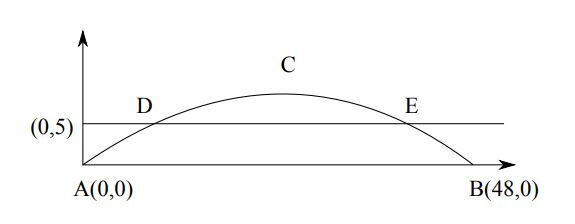
\includegraphics[width=0.7\linewidth]{images/Q8a}
\end{figure}
\vspace{-0.7cm}
\begin{enumerate}[(i)]
\item Using the coordinate plane, with A(0, 0) and B(48, 0), the equation of
the parabola is $y = −0.013x^2 + 0.624x$.\\
Find the coordinates of $C$, the highest point of the arch.
\item  The perpendicular distance between the walking deck, $[DE]$, and $[AB]$
is 5 metres.
Find the coordinates of $D$ and of $E$. \\ Give your answers correct to the
nearest whole number.
\item  Using integration, find the area of the shaded region, $ABED$, shown
in the diagram below.\\
Give your answer correct to the nearest whole number.
\begin{figure}[h!]
	\centering
	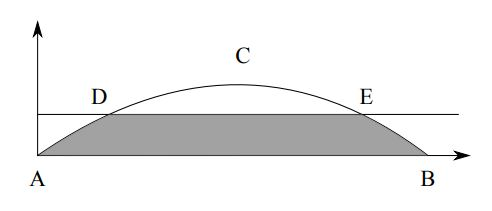
\includegraphics[width=0.7\linewidth]{images/Q8b}
\end{figure}
\vspace{-0.9cm}
\item  Write the equation of the parabola in part (i) in the form
$y - k = p(x - h)^2,$ where $k$, $p$ and $h$ are constants.
\item  Using what you learned in part (iv) above, or otherwise, write down
the equation of a parabola for which the coefficient of $x^2$
is $-2$ and
the coordinates of the maximum point are $(3, -4)$.
\end{enumerate}
\subsection*{Question 9}

\begin{itemize}

\item[(a)] The cost \euro $C$ of running a ship per hour is given by

$$ C = 4 + \frac{ V^3}{2500},$$

where $V$ is the speed in knots through the water.
\begin{enumerate}[(i)]
	\item What is the most economical speed through the water at which a voyage can be made against a current of 5 knots?
	\item Calculate the minimum cost to the nearest 10 euro?
	\item Sketch the graph of the cost ($C$) versus the speed ($V$) in the interval $0 < V < 20$.
\end{enumerate}
\item[(b)]
Oil is poured into a cylindrical tank of radius 1.2m, length 2.4 m with its axis horizontal.
When the depth of the oil is 0.6 m, the level of the oil is rising at the rate of 0.25cm per second.
How fast is the oil pouring into the tank? Give your answer in cubic meters per minute.


\end{itemize}
\end{document}
%=========================================%
\newpage\subsection*{Old Question 9}

\begin{itemize}


\item[(a)]

When a loan of $\euro P$ is repaid in equal repayments of amount $\euro A$, at the end of each of $t$ equal
periods of time, where $i$ is the periodic compound interest rate (expressed as a decimal), the formula below
can be used to find the amount of each repayment.

\[ A = P \frac{i(1+i)^t}{((1+i)^t -1)} \]
Show how this formula is derived. You may use the formula for the sum of a finite geometric series.

\item[(b)]
 Alex has a credit card $\euro 5000$. One method of clearing this debt is to make a fixed repayment at the end of each month.
	
\begin{enumerate}[(i)]
\item What is the fixed monthly repayment, $\euro A$, required to repay the debt of $\euro 5000$.
\item The annual percentage (APR) charged on debt by the credit card company is $21.75\%$, fixed for the term of the debt.
Find as a percentage, correct to 3 significant figures, the monthly interest rate that is equivalent to an APR of $21.75\%$.
\item Assume Alex pays the fixed monthly repayment $\euro A$, each month and does not have any further transactions on that card.
Complete the table below to show how the balance of the debt $\euro 5000$ is reducing each month for the first three months, assuming
an APR of $21.75\%$, charged and compounded monthly.
\\
\medskip
\begin{center}
	\begin{tabular}{|c|c|c|c|c|}
		\hline 

		Payment  & Fixed Monthly & Interest & Previous Balanced & Newblance  \\ 
		\hline 
		Number & Payment (A) &  & Reduced by (\$) & debt \\ 
		\hline \hline
		0 &  &  &  & 5000 \\ 
		\hline 
		1 &  &  & 42.50 & 4957.50 \\ 
		\hline 
		2 &  &  &  &  \\ 
		\hline 
		3 &  &  &  &  \\ 
		\hline 
	\end{tabular} 
\end{center}
\newpage
	\item Using the formulae that you derived on the previous page or otherwise, find how long it would take to pay off a credit 
card of $\euro 5000$, using the repayment method outlined at the beginning of \textbf{part (b)} above.
Give your answer in months, correct to the nearest month.

\item Alex decides to borrow $\euro 5000$ from the local Credit Union to pay off this credit card debt of $\euro 5000$.
The APR charge for the Credit Union Loan is $8.5\%$ fixed for the term of the loan. The loan is to be repaid in equal weekly repayments, at the
end of each week, for 156 weeks. Find the amount of each weekly repayment.
\end{enumerate}

\end{itemize}

\end{document}
